\chapter{Explainability in Deep Learning} 
\label{sec:Explainability} 

Machine Learning systems and especially Deep Neural Networks have the property that they are often seen as ``black-boxes'' \ie they are hard to interpret and pinpointing as a user how and why they recommend a certain course of action is often very difficult, if not impossible. This property becomes a prominent impediment for intelligent systems deployed in impactful sectors like, for example, employment \citep{QinZXZJCX18, CaiSJLQXZ20, ZhaoHCFZ18}, jurisdiction \citep{GuoHQX019}, healthcare \citep{Pasa2019}, or banking loans where users would like to know the deciding factors for decisions. As such, we would like systems that are easily interpretable, relatable to the user, provide contextual information about the choice, and reflect the intermediate thinking of the user for a decision \citep{xie2020explainable}. Since these properties are very broad, it is not surprising that researchers in this field have very different approaches \citep{xie2020explainable}. For this chapter, we utilized the field guide by \citet{xie2020explainable} to paint an appropriate overview and properly explain the different approaches. Commonly, methods try to provide better solutions regarding the traits \emph{Confidence}, \emph{Trust}, \emph{Safety}, and \emph{Ethics} to improve the overall explainability of the system \citep{xie2020explainable}:

\paragraph{Confidence}
This trait is increasing when the ``reasoning'' behind a decision between the DNN and the user matches. Hence, for example, saliency attention maps \citep{ParkHARSDR18, HudsonM18} ensure that semantically loaded parts of an image get considered and therefore increase confidence.

\paragraph{Trust} 
Trust is established when the decision of the intelligent system doesn't need to be validated. Recently, many works have studied the problem whether a model can safely be adopted \citep{GharibLBADB18, VarshneyA17, JiangKGG18}. To be able to trust a model, we need to ensure \emph{satusfactory testing} of the model as well as \emph{experience} with the model to ensure that the results commonly match the expectation as data drifts \citep{xie2020explainable}.

\paragraph{Safety}
Safety needs to be high for intelligent systems that impact human life in any form. As such, the model should perform \emph{consistently} as expected, \emph{prevent} choices that have a negative impact on the user or society, have a high \emph{reliability} under all operating conditions, and provide \emph{feedback} on how the operating conditions influence the behavior \citep{xie2020explainable}.

\paragraph{Ethics}
This trait is defined differently depending on the moral principles of each user. In general, though, one can create an ``ethics code'' which a system's decisions are based off \citep{xie2020explainable}. One example is that try to prevent racial biases or reduce the effect of any features that serves as a proxy for this type of discrimination process. Similarly, any protected characteristic \eg  religion, gender, disability, or sexual orientation are features which should be handled with great care.


\section{Related topics}
There exist several concepts which are related to explainable deep learning. Here, we cover \emph{model debugging} which tries to identify aspects which hinder training inference, \emph{fairness and bias} which especially tackles the ethics trait, and \emph{adversarial attack and defense} which search for differences in regular and irregular activation patterns to promote robust and trustworthy systems \citep{xie2020explainable}. 

\subsection{Model Debugging}
\emph{Model debugging}, similar to traditional software debugging, tries to pinpoint aspects of the architecture, data-processing, or training process which cause errors \citep{xie2020explainable}. 

\citet{amershi2015modeltracker} propose \textsc{ModelTracker} which is a debugging framework and interactive visualization that displays traditional statistics like Area Under the Curve (AUC) or confusion matrices. It also shows how close samples are in the feature space and allows users to expand the visualization to show the raw data or annotate them. \citet{AlainB17} deploy linear classifiers to predict the information content in intermediate layers where the features of every layer serve as input to the separate classifier. They show that using features from deeper layers improves prediction accuracy and  that level of linear separability increases monotonically. \citet{fuchs2018scrutinizing} introduce \emph{neural stethoscopes} as a framework for analyzing factors of influence and interactively promoting and suppressing information. They extend the ordinary DNN architecture via a parallel two layer perceptron at different locations where the input are the features from any layer from the main architecture. This stethoscope is then trained on a supplemental task and the loss is back-propagated to the main model with weighting factor $\lambda$ \citep{fuchs2018scrutinizing}. This factor controls if the stethoscope functions analytical ($\lambda = 0$), auxiliary ($\lambda > 0$), or adversarial ($\lambda < 0$) \citep{fuchs2018scrutinizing}. Further, \citet{KangRBZ20} use \emph{model assertions} which are functions for a model's input and output that indicate when errors may be occurring. They show that with these they are able to solve problems where car detection in successive frames disappears and reappears \citep{KangRBZ20}. Model debugging is therefore implemented through a verification system \citep{xie2020explainable}. 

%\subsection{Adversarial Attack and Defense}

\subsection{Fairness and Bias}
To secure \emph{model fairness}, there exist several definitions which have emerged in the literature in recent years. \emph{Group fairness} \citep{CaldersKP09}, also known as  demographic parity or statistical party, aims at equalizing benefits across groups with respect to protected characteristics (\eg religion, gender, etc.). By definition, if group $A$ has twice as many people as group $B$, twice as many people in group $A$ should receive the benefit when compared to $B$ \citep{xie2020explainable}. On the other hand, \emph{individual fairness} \citep{DworkHPRZ12} tries to secure that similar inputs get treated similarly. There also exist other notions of fairness such as \emph{equal opportunity} \citep{HardtPNS16}, \emph{disparate mistreatment} \citep{ZafarVGG17}, or other variations \citep{HeidariFGK18, WoodworthGOS17}.

Methods which try to tackle fairness can be classified into three approaches called \emph{pre-processing}, \emph{in-processing}, \emph{post-processing}:
\begin{enumerate}
    \item \textbf{Pre-processing} methods adapt the input data beforehand to remove features correlated to protected characteristics. As such, they try to learn an alternative feature representation without these attributes \citep{GordalizaBGL19, CalmonWVRV17, LouizosSLWZ15, ZemelWSPD13}. 
    \item \textbf{In-processing} approaches add adjustments for fairness in the model learning process. This way, they punish decisions which are not aligned with certain fairness constraints \citep{DworkIKL18, DoniniOBSP18, AgarwalBD0W18}.
    %\citep{DworkIKL18, DoniniOBSP18, MenonW18, AgarwalBD0W18}
    \item \textbf{Post-processing} methods adjust the model predictions afterwards to account for fairness. It is the reassignment of class labels after classification with the goal of minimizing 
    classification errors subject to a particular fairness constraint \citep{HardtPNS16,PleissRWKW17, FeldmanFMSV15}.
\end{enumerate}


\section{Previous Works}

\citep{BargalZKZMS18} \citep{SelvarajuCDVPB20} \citep{SimonyanVZ13} \citep{ZhangBLBSS18} \citep{ChenLTBRS19} 
\citep{CaoLYYWWHWHXRH15} \citep{SelvarajuLSJGHB19} \citep{RossHD17}

Spatial semantic segmentation: \citep{LiWPE018} \citep{ZhouZYQJ18} \citep{WeiFLCZY17}

Object localization: \citep{ZhangWF0H18}

 Prototypes: \citep{LiLCR18}
 
 Generally, we can divide methods for explainable deep neural networks in \emph{visualization}, \emph{model distillation}, and \emph{intrinsic} methods \citep{xie2020explainable}. While \emph{visualization} methods try to highlight features which strongly correlate with the output of the DNN, \emph{model distillation} builds upon a jointly trained ``white-box'' model, following the input-output behavior of the original architecture and aiming to identify its decision rules \citep{xie2020explainable}. Finally, \emph{intrinsic} methods are networks designed to explain their output, hence they aim to optimize both, its performance and the respective explanations \citep{xie2020explainable}.

\subsection{Visualization}
Commonly, visualization methods use saliency maps to display the saliency values of the features \ie to which degree the features influence the model's prediction \citep{xie2020explainable}. We can further divide visualization methods into \emph{back-propagation} and \emph{perturbation} based approaches where they respectively determine these values based on the volume of the gradient or between modified versions of the input \citep{xie2020explainable}. 

\subsubsection{Back-Propagation}
These approaches stick to the gradient passed through the network to determine the relevant features. As a simplistic baseline, one can display the partial derivative with respect to each input feature multiplied by its value \citep{xie2020explainable}. This way,  \citet{SimonyanVZ13} and \citet{SpringenbergDBR14} assess the sensitivity of the model for input changes \citep{xie2020explainable}. This can also be done for collections of intermediate layers \citep{ShrikumarGK17, MontavonLBSM17, Bach2015, ZeilerF14}.

\citet{ZhouKLOT16} introduce class activation maps (CAMs) which are shown in \Cref{fig:cams} based on global average pooling (GAP) \citep{LinCY13}. With GAP, they deploy the following CNN structure at the end of the network: \texttt{GAP(Convs)} $\rightarrow$ \texttt{Fully Connected Layer (FC)} $\rightarrow$ \texttt{softmax} \citep{LinCY13} where CAMs $M_{c}$ for each class are then calculated according to \Cref{eq:cam}. Here, $K$ are convolutional filters, $\mathbf{A}$ are the activations of the last convolutional layer, and $ w_{k, c}$ indicate the weights from the \texttt{Conv} to the \texttt{FC} \citep{ZhouKLOT16}.
\begin{equation}
\label{eq:cam}
    M_{c}=\sum_{k}^{K} w_{k, c} \mathbf{A}_{k}
\end{equation}
By upsampling the map to the image size, they are able to visualize the image regions responsible for a certain class \citep{ZhouKLOT16}. Therefore, every class has it's own individual class activation map. 
\begin{figure}[htbp]
    \centering
    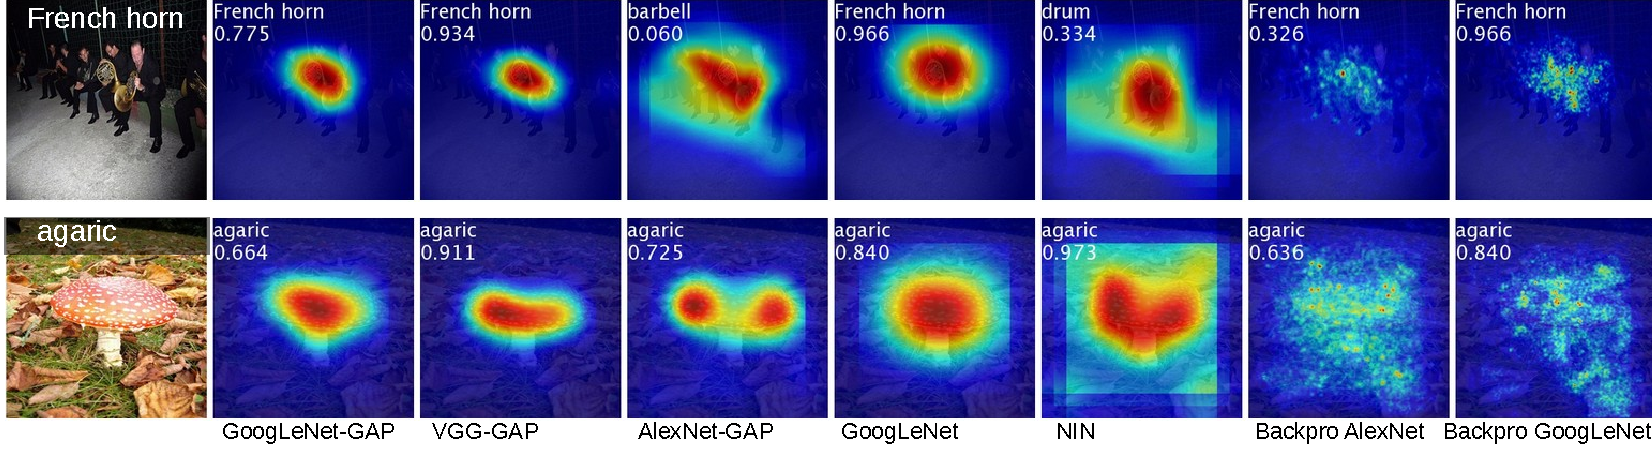
\includegraphics[width=\textwidth]{Figures/Chapter3/heatmapAll.pdf}
    \caption[CAMs across different architectures]{CAMs across different architectures: \citep{ZhouKLOT16}}
    \label{fig:cams}
\end{figure}
The drawback of their approach is, that their method can only be applied to networks which use the \texttt{GAP(Convs)} $\rightarrow$ \texttt{Fully Connected Layer (FC)} $\rightarrow$ \texttt{softmax} architecture at the end \citep{xie2020explainable}. 

\citet{SelvarajuCDVPB17} solve this by generalizing the CAMs to gradient-weighted class activation maps (Grad-CAMs). Since their approach only requires a the final activation function to be differentiable, they are generally applicable to a broader range of CNN architectures \citep{SelvarajuCDVPB17, xie2020explainable}. For that, they compute an importance score $\alpha_{k,c}$ shown in \Cref{eq:grad_cam_importance}.
\begin{equation}
\label{eq:grad_cam_importance}
    \alpha_{k,c} = \frac{1}{m\cdot n}\sum_{i=1}^m\sum_{j=1}^n \frac{\partial y_c}{\partial \mathbf{A}_{k,i,j}}
\end{equation}
Here, $y_c$ is the score before \texttt{softmax} and we calculate the gradient with respect to the feature map $\mathbf{A}_k$ in the final convolutional layer for every neuron positioned at $(i,j)$ in the $m\times n$ feature map \citep{SelvarajuCDVPB17, xie2020explainable}. Afterwards, these importance scores get linearly combined for every feature map as shown in \Cref{eq:grad_cam_map} where they get additionally passed through a \texttt{ReLU} function.
\begin{equation}
\label{eq:grad_cam_map}
    M_c = \operatorname{ReLU}\Big(\sum_k^K \alpha_{k,c} \mathbf{A}_k \Big)
\end{equation}
This computation inherently yields a $m \times n$ importance map ($14 \times 14$ for VGG \citep{SimonyanZ14a} and AlexNet \citep{KrizhevskySH12}) where we upsample it using bilinear interpolation onto the image size to yield the Grad-CAM.

Apart from CAMs, there also exist other methods like layer-wise relevance propagation \citep{MontavonLBSM17, DingLLS17, LapuschkinBMMS16, Bach2015}, deep learning important features (DeepLIFT) \citep{ShrikumarGK17}, or integrated gradients \citep{SundararajanTY17} which are not described in detail here. Refer to \citet{xie2020explainable} or the original works for more information.

\subsubsection{Perturbation}
Methods that build upon perturbation alternate the input features to compute their respective relevance for the model's output by comparing the differences between the original and permutation.

\citet{ZeilerF14} sweep a gray patch over the image to determine how the model will react to occluded areas. Once, an area with high correlation to the output is covered, the prediction performance drops \citep{xie2020explainable, ZeilerF14}. \citet{li2016understanding} deploy a similar idea for NLP tasks where they erase words and measure the influence on the model's performance. \citet{FongV17}



\subsection{Model distillation}
\subsubsection{Local approximations}
\subsubsection{Model Translation}

\subsection{Intrinsic methods}
\subsubsection{Attention Mechanisms}
\subsubsection{Joint Training}

\section{Explainability for Domain Generalization}

\citep{zunino2020explainable}